\documentclass[12pt, a4paper]{article}

\newcommand{\kafedra}{ИИТ} % Кафедра X

\newcommand{\numberOfLab}{2} % Лабораторная работа №X
\newcommand{\semestr}{2} % За X семестр
\newcommand{\distiplina}{ОАиП} % По дисциплине <<X>>
\newcommand{\labTitle}{Пользовательские функции} % Тема: <<X>>

% Выполнил
\newcommand{\kurs}{1} % Студент X курса
\newcommand{\group}{ПО-4 (1)} % группы X
\newcommand{\labAuthor}{Галанин П. И.} % X

% Проверил
\newcommand{\teacherStatus}{ст. преподаватель} % X
\newcommand{\teacher}{Хацкевич М. В.} % X

\newcommand{\labDate}{Брест, 2020} % X

\usepackage{../../sty/encoding} % кодировка
\usepackage{../../sty/titlePage} % титульный лист
\usepackage{../../sty/fields} % поля
\usepackage{../../sty/imgs} % картинки
\usepackage{../../sty/code} % исходный код
\usepackage{../../sty/labData} % для лабораторной

\begin{document}

% титульный лист
\maketitle
\setcounter{page}{2}

% содержание
\renewcommand{\contentsname}{Содержание}
\tableofcontents
\newpage

% контент
\labheading

\labgoal{Изучить основные принципы написания пользовательских функций, ознакомиться с возможностями передачи данных в функции и получения результата по итогам работы функции. Реализовать собственные функции для обработки данных составных и простых типов.}

\labreport

\section{Задание A}

\subsection{Условие}

\begin{center}
    \textbf{Вариант 25}
\end{center}

Описать процедуру Transp(A, M), выполняющую транспонирование (то есть зеркальное отражение относительно главной диагонали) квадратной вещественной матрицы A порядка M. Матрица A является входным и выходным параметром. Используя эту процедуру, транспонировать данную матрицу A порядка M.

\subsection{Структура проекта}

\begin{verbatim}
.
├── Makefile
├── inc     
│   ├── generate_matrix.h
│   ├── integer_swap.h   
│   ├── lab.h
│   ├── main.h
│   ├── print_matrix.h   
│   └── transp_matrix.h  
└── src
    ├── generate_matrix.c
    ├── integer_swap.c   
    ├── lab.c
    ├── main.c
    ├── print_matrix.c
    └── transp_matrix.c
\end{verbatim}

\subsection{Исходный код}

\subsubsection{Makefile}
\lstinputlisting[language=make]{a/25/Makefile}

\subsubsection{main()}
Блоксхема на рисунке \ref{fig:a_25_main}.
\lstinputlisting[language=C]{a/25/inc/main.h}
\lstinputlisting[language=C]{a/25/src/main.c}

\subsubsection{lab()}
Блоксхема на рисунке \ref{fig:a_25_lab}.
\lstinputlisting[language=C]{a/25/inc/lab.h}
\lstinputlisting[language=C]{a/25/src/lab.c}

\subsubsection{generate\_matrix()}
Блоксхема на рисунке \ref{fig:a_25_generate_matrix}.
\lstinputlisting[language=C]{a/25/inc/generate_matrix.h}
\lstinputlisting[language=C]{a/25/src/generate_matrix.c}

\subsubsection{print\_matrix()}
Блоксхема на рисунке \ref{fig:a_25_print_matrix}.
\lstinputlisting[language=C]{a/25/inc/print_matrix.h}
\lstinputlisting[language=C]{a/25/src/print_matrix.c}

\subsubsection{transp\_matrix()}
Блоксхема на рисунке \ref{fig:a_25_transp_matrix}.
\lstinputlisting[language=C]{a/25/inc/transp_matrix.h}
\lstinputlisting[language=C]{a/25/src/transp_matrix.c}

\subsubsection{integer\_swap()}
Блоксхема на рисунке \ref{fig:a_25_integer_swap}.
\lstinputlisting[language=C]{a/25/inc/integer_swap.h}
\lstinputlisting[language=C]{a/25/src/integer_swap.c}

\subsection{Исполняемая программа}

\begin{verbatim}
Размер квадратной матрицы: 5
2       8       1       8       6
8       2       4       7       2
6       5       6       8       6
5       7       1       8       2
9       9       7       7       9

Транспонированная матрица:
2       8       6       5       9
8       2       5       7       9
1       4       6       1       7
8       7       8       8       7
6       2       6       2       9
\end{verbatim}

\labconclusion{}

\newpage

% Задание B - - - - - - - - - -
\section{Задание B}

\subsection{Условие}

\begin{center}
    \textbf{Вариант 7}
\end{center}

Описать функцию $InvertStr(S, K, N)$ строкового типа, возвращающую инвертированную подстроку строки $S$, содержащую в обратном порядке $N$ символов строки $S$, начиная с ее $K$-го символа. Если $K$ превосходит длину строки $S$, то возвращается пустая строка; если длина строки меньше $K + N$, то инвертируются все символы строки, начиная с ее $K$-го символа. Вывести значения функции $InvertStr$ для данной строки $S$ и каждой из трех пар положительных целых чисел: $(K1, N1), (K2, N2), (K3, N3)$.

\subsection{Структура проекта}

\begin{verbatim}
.
├── Makefile
├── inc
│   ├── char_swap.h
│   ├── get_invert_string.h
│   ├── lab.h
│   └── main.h
└── src
    ├── char_swap.c
    ├── get_invert_string.c
    ├── lab.c
    └── main.c
\end{verbatim}

\subsection{Исходный код}

\subsubsection{Makefile}
\lstinputlisting[language=make]{b/7/Makefile}

\subsubsection{main()}
Блоксхема на рисунке \ref{fig:b_7_main}.
\lstinputlisting[language=C]{b/7/inc/main.h}
\lstinputlisting[language=C]{b/7/src/main.c}

\subsubsection{lab()}
Блоксхема на рисунке \ref{fig:b_7_lab}.
\lstinputlisting[language=C]{b/7/inc/lab.h}
\lstinputlisting[language=C]{b/7/src/lab.c}

\subsubsection{get\_inverting\_string()}
Блоксхема на рисунке \ref{fig:b_7_get_invert_string}.
\lstinputlisting[language=C]{b/7/inc/get_invert_string.h}
\lstinputlisting[language=C]{b/7/src/get_invert_string.c}

\subsubsection{char\_swap()}
Блоксхема на рисунке \ref{fig:b_7_char_swap}.
\lstinputlisting[language=C]{b/7/inc/char_swap.h}
\lstinputlisting[language=C]{b/7/src/char_swap.c}

\subsection{Исполняемая программа}

\begin{verbatim}
Размер строки: 100
Строка: 0123456789
С какого символа: 2
Сколько символов: 6
Изменённая строка: 0176543289
\end{verbatim}

\labconclusion{}

\newpage

% Задание С - - - - - - - - - -
\section{Задание C}

\subsection{Условие}

\begin{center}
    \textbf{Вариант 7}
\end{center}

Описать рекурсивную функцию $Combin2(N, K)$ целого типа, находящую $C(N, K)$ — число сочетаний из $N$ элементов по $K$ — с помощью рекуррентного соотношения:

$C(N, 0) = C(N, N) = 1$,

$C(N, K) = C(N - 1, K) + C(N - 1, K - 1)$

при $0 < K < N$.

Параметры функции — целые числа; $N > 0$, $0 \leq K \leq N$. Считать, что параметр $N$ не превосходит $20$. С помощью функции Combin2 найти числа $C(N, K)$ для данного значения N и пяти различных значений K.

\subsection{Структура проекта}

\begin{verbatim}
.
├── Makefile
├── inc
│   ├── Combin2.h
│   ├── lab.h
│   └── main.h
└── src
    ├── Combin2.c
    ├── lab.c
    └── main.c
\end{verbatim}

\subsection{Исходный код}

\subsubsection{Makefile}
\lstinputlisting[language=make]{c/7/Makefile}

\subsubsection{main()}
Блоксхема на рисунке \ref{fig:c_7_main}.
\lstinputlisting[language=C]{c/7/inc/main.h}
\lstinputlisting[language=C]{c/7/src/main.c}

\subsubsection{lab()}
Блоксхема на рисунке \ref{fig:c_7_lab}.
\lstinputlisting[language=C]{c/7/inc/lab.h}
\lstinputlisting[language=C]{c/7/src/lab.c}

\subsubsection{Combin2()}
Блоксхема на рисунке \ref{fig:c_7_Combin2}.
\lstinputlisting[language=C]{c/7/inc/Combin2.h}
\lstinputlisting[language=C]{c/7/src/Combin2.c}

\subsection{Исполняемая программа}

\begin{verbatim}
Сколько элементов: 6
Сколько раз: 3    
Combin2(6, 3) = 20

Сколько элементов: 5
Сколько раз: 3
Combin2(5, 3) = 10

Сколько элементов: 4
Сколько раз: 3
Combin2(4, 3) = 4

Сколько элементов: 3
Сколько раз: 3
Combin2(3, 3) = 1

Сколько элементов: 2
Сколько раз: 3
Combin2(2, 3) = -1

Сколько элементов: 1
Сколько раз: 3
Combin2(1, 3) = -1
\end{verbatim}

\labconclusion{}

\newpage

\section{Приложения}

\begin{figure}[h]
    \center{
        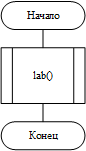
\includegraphics[]{a/25/flowcharts/main.png}
    }
    \caption{main()}
    \label{fig:a_25_main}
\end{figure}

\begin{figure}[h]
    \center{
        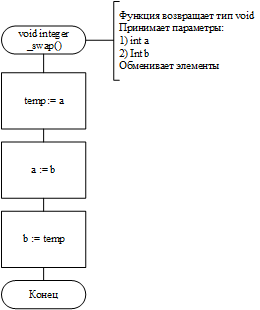
\includegraphics[]{a/25/flowcharts/integer_swap.png}
    }
    \caption{integer\_swap()}
    \label{fig:a_25_integer_swap}
\end{figure}

\begin{figure}[h]
    \center{
        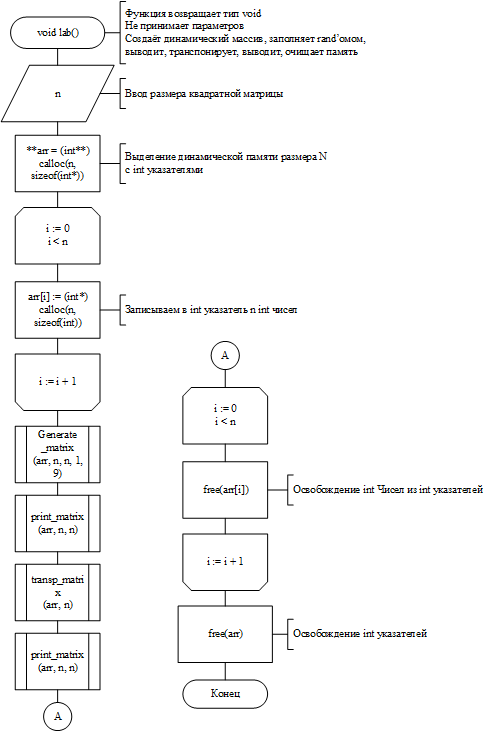
\includegraphics[]{a/25/flowcharts/lab.png}
    }
    \caption{lab()}
    \label{fig:a_25_lab}
\end{figure}

\begin{figure}[h]
    \center{
        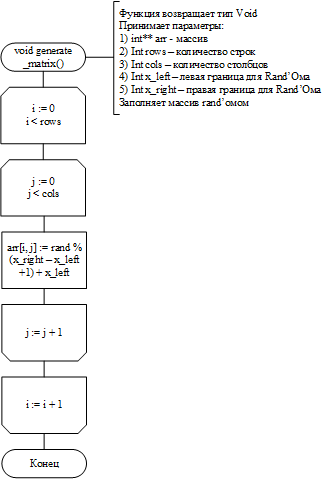
\includegraphics[]{a/25/flowcharts/generate_matrix.png}
    }
    \caption{generate\_matrix()}
    \label{fig:a_25_generate_matrix}
\end{figure}

\begin{figure}[h]
    \center{
        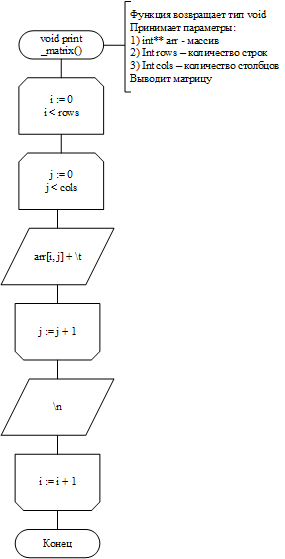
\includegraphics[]{a/25/flowcharts/print_matrix.png}
    }
    \caption{print\_matrix()}
    \label{fig:a_25_print_matrix}
\end{figure}

\begin{figure}[h]
    \center{
        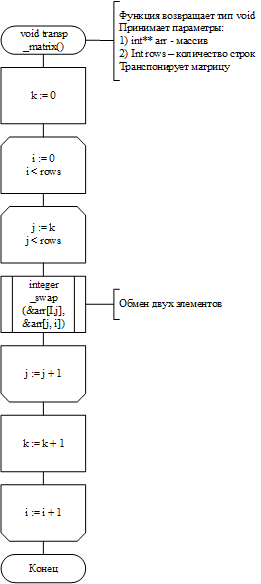
\includegraphics[]{a/25/flowcharts/transp_matrix.png}
    }
    \caption{transp\_matrix()}
    \label{fig:a_25_transp_matrix}
\end{figure}

\begin{figure}[h]
    \center{
        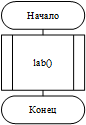
\includegraphics[]{b/7/flowcharts/main.png}
    }
    \caption{main()}
    \label{fig:b_7_main}
\end{figure}

\begin{figure}[h]
    \center{
        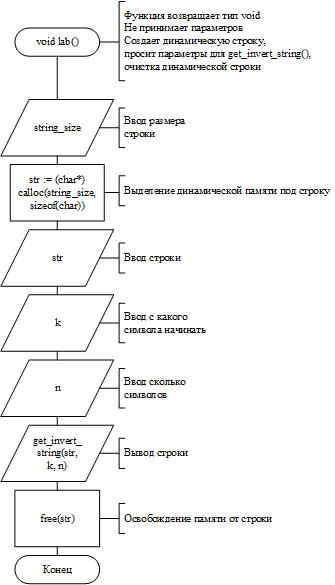
\includegraphics[]{b/7/flowcharts/lab.png}
    }
    \caption{lab()}
    \label{fig:b_7_lab}
\end{figure}

\begin{figure}[h]
    \center{
        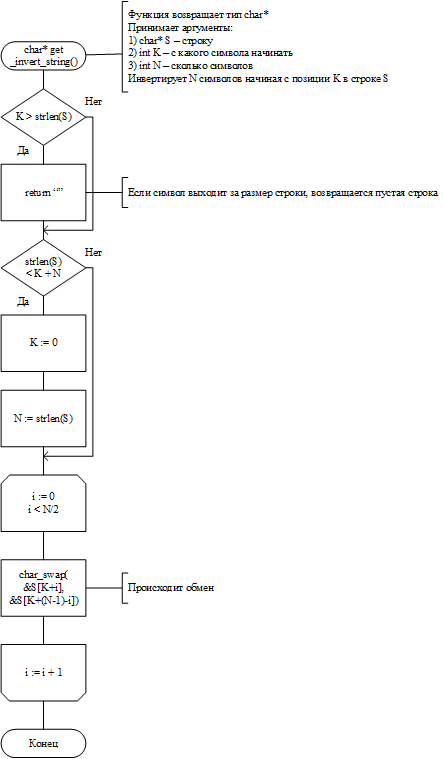
\includegraphics[]{b/7/flowcharts/get_invert_string.png}
    }
    \caption{get\_invert\_string()}
    \label{fig:b_7_get_invert_string}
\end{figure}

\begin{figure}[h]
    \center{
        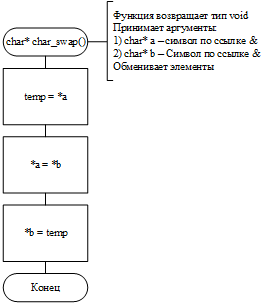
\includegraphics[]{b/7/flowcharts/char_swap.png}
    }
    \caption{char\_swap()}
    \label{fig:b_7_char_swap}
\end{figure}

\begin{figure}[h]
    \center{
        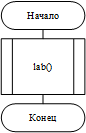
\includegraphics[]{c/7/flowcharts/main.png}
    }
    \caption{main()}
    \label{fig:c_7_main}
\end{figure}

\begin{figure}[h]
    \center{
        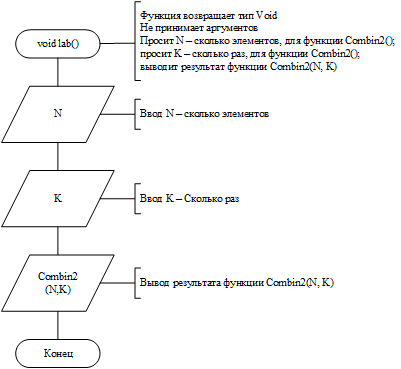
\includegraphics[]{c/7/flowcharts/lab.png}
    }
    \caption{lab()}
    \label{fig:c_7_lab}
\end{figure}

\begin{figure}[h]
    \center{
        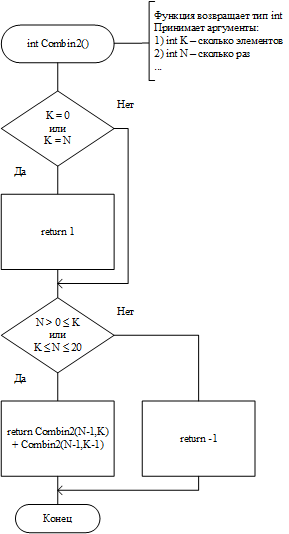
\includegraphics[]{c/7/flowcharts/Combin2.png}
    }
    \caption{Combin2()}
    \label{fig:c_7_Combin2}
\end{figure}

\end{document}